\documentclass{article}
\usepackage{parskip}
\usepackage{fullpage}
\usepackage{amsmath}
\usepackage{amssymb}
\usepackage{latexsym,paralist}
\usepackage{comment}
\usepackage{fancyvrb}
\usepackage{graphicx}
\usepackage{tikz}
\usetikzlibrary{arrows.meta}
\pagestyle{empty}

\includecomment{solution}
\excludecomment{solution}  % comment this out to create the solutions

\newcommand{\bs}{\noindent\textbf{Solution.}~}
\newcommand{\es}{\hfill $\square$}

\setcounter{secnumdepth}{-1}

\begin{document}
\subsection{IE 5545 A Network Game of Compliments}
In a game of compliments a player has an increasing incentive to choose an action as
more neighbors choose the action. Suppose that there are only two actions for each player,
0 or 1. A player $i$ will choose action 1 if the number of neighbors taking action 1 meets
or exceeds some threshold $t_i$. The utility of player $i$ obeys
\[ u_i(1,S_{N_i}) \geq u_i(0,S_{N_i}) \quad \text{if and only if}
  \quad \sum_{j \in N_i} a_j \geq t_i \]
where $N_i$ are the neighbors
of player $i$, $S_{N_i}$ are the strategies of the neighbors of player $i$,
$a_j$ is the action taken by player j, and $t_i$ is the threshold
for player $i$. Find a pure strategy Nash equilibrium for the game of compliments
shown below that is different from either of the two equilibriums
given in class for this game. The threshold is 2.

\vspace{.5in}
\begin{center}
\resizebox{.7\textwidth}{!}{%
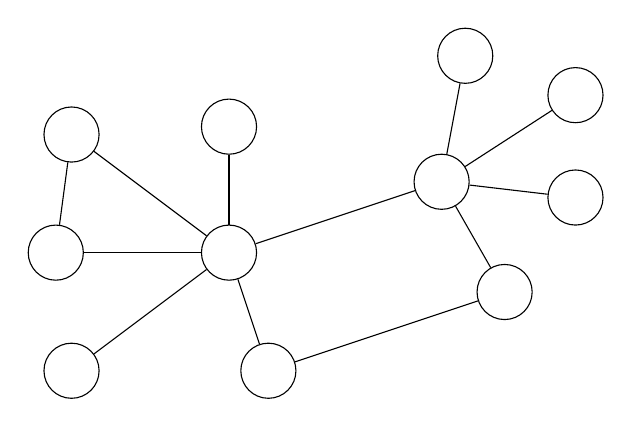
\begin{tikzpicture}
  \tikzstyle{every circle node}=[draw,inner sep=0pt,minimum size=7mm]
  
  \draw (0,0) node[circle] (A) {};
  \draw (2.7,.9) node[circle] (B) {};

  \draw (0,1.6) node[circle] (C) {};
  \draw (-2,1.5) node[circle] (D) {};
  \draw (-2.2,0) node[circle] (E) {};
  \draw (-2,-1.5) node[circle] (F) {};
 
  \draw (3,2.5) node[circle] (G) {};
  \draw (4.4,2) node[circle] (H) {};
  \draw (4.4,.7) node[circle] (I) {};
  \draw (3.5,-.5) node[circle] (J) {};
  \draw (.5,-1.5) node[circle] (K) {};

  \path (A) edge (B);
  \path (A) edge (C);
  \path (A) edge (D);
  \path (A) edge (E);
  \path (A) edge (F);
  \path (A) edge (K);

  \path (B) edge (G);
  \path (B) edge (H);
  \path (B) edge (I);
  \path (B) edge (J);

  \path (J) edge (K);
  \path (D) edge (E);

\end{tikzpicture}
}%
\end{center}

\end{document}
